\begin{enumerate}
\item Why would we want to know what a circuit's \thev Equivalent circuit is?
\item What are the two components of a \thev Equivalent circuit?
\item Think about the two-stage amplifier that you built in Chapter~\ref{chapTransVoltageAmp}.  How would you go about finding the \thev Equivalent circuit as it is seen by the headphones?
\item Suppose I have a circuit where the output terminals have a $2\myvolt$ drop when it is an open circuit, and have $2\mymamp$ of current flowing through it when it is a short circuit.  Draw the \thev Equivalent circuit.
\item If I have a \thev Equivalent circuit of $4\myvolt$ with an impedance of $400\myohm$, what will be the voltage drop of the load if I attach a $2000\myohm$ resistor across the output?
\item If I have a \thev Equivalent circuit of $3\myvolt$ with an impedance of $100\myohm$, what will be the voltage drop, the current, and the power of the load if I attach headphones rated at $32\myohm$?
\item Calculate and draw the \thev Equivalent circuit of the circuit below: 
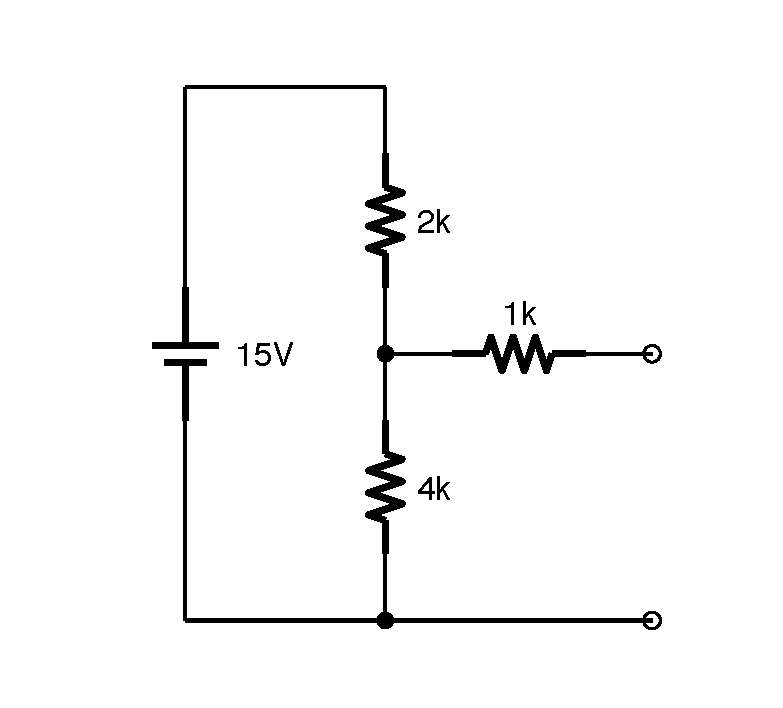
\includegraphics[scale=0.25]{ThevProblem1.pdf}
\item Suppose I have a circuit where, when I add a load of $350\myohm$ I get a $7\myvolt$ drop, and when I add a load of $2000\myohm$ I get an $8\myvolt$ drop.  Calculate and draw the \thev Equivalent circuit.
\end{enumerate}
